\documentclass[twocolumn]{article}
\usepackage{xeCJK}  %必须加xeCJK包
\setCJKmainfont{AR PL UMing CN}  %换成本地字体

\usepackage{times}
\usepackage{graphicx} % more modern
\usepackage{epstopdf}
\usepackage{subfigure} 
\usepackage{natbib}
\usepackage[boxed]{algorithm}
\usepackage{algorithmic}
\usepackage{hyperref}
\usepackage{framed}
\newcommand{\theHalgorithm}{\arabic{algorithm}}

\usepackage{amsmath}
\usepackage{array}
\usepackage{stackengine}

\usepackage[letterpaper, margin=1in, top=0.5in]{geometry}

\begin{document}


\newcommand{\jac}[2]{\frac{\partial #1}{\partial #2}}
\newcommand{\xhat}{\widehat{x}}
\newcommand{\yhat}{\widehat{y}}
\newcommand{\zhat}{\widehat{z}}
\newcommand{\vxhat}{\widehat\mathrm{x}}
\newcommand{\vzhat}{\widehat\mathrm{z}}
\newcommand{\setX}{\mathcal{X}}
\newcommand{\setB}{\mathcal{B}}
\newcommand{\E}{\text{E}}
\newcommand{\Var}{\text{Var}}
\newcommand{\Cov}{\text{Cov}}
\newcommand{\Fhat}{\widehat{F}}
\newcommand{\Thetahat}{\widehat{\Theta}}
\newcommand{\Norm}{\text{Norm}}
\newcommand{\BatchNorm}{\text{BN}}
\newcommand{\kk}{{(k)}}
\newcommand{\vx}{\mathrm{x}}
\newcommand{\vy}{\mathrm{y}}
\newcommand{\vz}{\mathrm{z}}
\newcommand{\vb}{\mathrm{b}}
\newcommand{\vu}{\mathrm{u}}
\newcommand{\comt}{// }
\renewcommand{\algorithmiccomment}[1]{\comt #1}
\newcommand{\BN}[2]{\text{BN}_{#2}(#1)}
\renewcommand{\algorithmicrequire}{\textbf{Input:}}
\renewcommand{\algorithmicensure}{\textbf{Output:}}
\newcommand{\mils}{\cdot 10^6}
\newcommand{\netw}[1]{{\sl #1}}
\newcommand{\norig}{\text{\sl N}}
\newcommand{\ntrain}{\norig_\mathrm{BN}^\mathrm{tr}}
\newcommand{\ninf}{\norig_\mathrm{BN}^\mathrm{inf}}
\setcitestyle{authoryear,round,citesep={;},aysep={,},yysep={;}}
\renewcommand{\cite}[1]{\citep{#1}}


\title{批量归一化:通过减少内部协变量转移加速深度网络训练}

\author{Sergey Ioffe \\Google Inc., {\sl sioffe@google.com} \and
Christian Szegedy \\Google Inc., {\sl szegedy@google.com} \and 翻译:Kenny(初),管枫(复),任远航(审)
}

\date{}

\maketitle

\begin{abstract}

在深度神经网络的训练过程中,先前层参数的调整会导致之后每一层输入值的分布发生变化,这种现象使模型的训练变得很复杂.所以在深度神经网络模型的训练中,通常需要仔细选取初始参数并采取较小的学习率,这不但导致模型训练的效率低下,而且使得饱和非线性模型的训练极为困难. 我们把这种现象称为内部协变量转移({\em
  internal covariate shift}),并通过归一化(normalizing)每层的输入来解决这个问题.  
我们方法的强大之处在于把归一化的步骤作为模型训练架构的一部分来实现, 并且对每个{\em 训练小批量}都执行归一化操作.
批量归一化允许我们使用很高的学习率并且对初始化不太在意.它在一定情况下也可以起到正则化的作用,并减轻了对Dropout的需求.我们在最先进的图像分类模型中使用批量归一化法,在减少了14倍训练步骤的情况下实现了与原模型相同的精度,并以显著增量击败了原始模型.我们使用批量归一化的网络模型,增强了在ImageNet分类上发布的最佳结果:获得了4.9\%前5验证误差(和4.8\%测试误差),这超出了人类评估者的准确率
\end{abstract}

\section{Introduction}

深度学习极大地提升了视觉,语言和许多其他领域。随机梯度下降(SGD)已经被证明是训练神经网络的一个有效的方法,并且随机梯度下降变种方法如动量\cite{momentum}和Adagrad\cite{momentum}已经被用来获得最先进的性能。随机梯度下降优化网络的参数$\Theta$,以便最小化损失
$$\Theta = \arg \min_\Theta
\frac{1}{N}\sum_{i=1}^N \ell(\vx_i, \Theta)$$
其中$\vx_{1\ldots N}$是训练集。在训练的每一步中我们考虑一个大小为$m$的小批量。这个小批量被用来近似相关联参数的损失函数的梯度,通过计算
$$\frac{1}{m} \jac{ \ell(\vx_i, \Theta)}{ \Theta}.$$
使用小批量的样本,而不是一次一个样本,有几点好处。首先,小批量上的损失梯度是训练集上梯度的一个估计,其质量随着批量大小的增加而提高。第二,由于现代计算平台提供的并行性,对一个批量$m$的计算比每个样本的$m$次计算更有效

虽然随机梯度是简单有效的,但是它需要仔细调整模型超参数,特别是使用在优化中的学习率以及模型参数的初始值。由于每层的输入受所有先前层的参数影响的事实,使训练复杂化,以致于网络参数的小变化随着网络变得更深而放大。

由于层需要不断地适应新的分布,层输入的分布的变化提出了一个问题。当一个学习系统的输入分布改变时,也就认为经历了{\em 协变量移位}\cite{covariate-shift},这个通常通过域适应(domainadaptation)\cite{domain-adaptation-survey}来处理。
但是,协变量移位的概念可以作为一个整体延伸超出学习系统,适用于他自身的部分,比如子网络或者一个层。
考虑一个计算如下损失函数的网络:$$\ell = F_2(F_1(\vu, \Theta_1), \Theta_2)$$ 其中
$F_1$ 和 $F_2$ 可以是任意变换, 网络通过训练参数
$\Theta_1, \Theta_2$ 来最小化损失函数 $\ell$.
对 $\Theta_2$ 的学习可以被看做以
$\vx=F_1(\vu,\Theta_1)$ 为输入,以
$$\ell = F_2(\vx, \Theta_2).$$ 为损失函数的独立网络。比如,梯度下降步骤
$$\Theta_2\leftarrow \Theta_2 - \frac{\alpha}{m}\sum_{i=1}^m
\jac{F_2(\vx_i,\Theta_2)}{\Theta_2}$$ (批量大小为 $m$ 学习率
为 $\alpha$) 完全等同于一个输入为$F_2$的独立网络$\vx$.  
因此,输入分布的属性使得训练更有效 -- 比如在训练和测试数据之间有相同的分布 -- 也适用于子网络的训练。
因此有利于$\vx$的分布随时间保持不变,同时$\Theta_2$不必不断调整来适应$\vx$分布的变化.

固定一个子网络输入的分布将对子网络外的层产生积极的影响。
用一个sigmoid激活函数$\vz = g(W\vu+\vb)$考虑一个层,其中$\vu$是层输入,权重矩阵$W$和阈值向量$\vb$是学习的层参数,$g(x) = \frac{1}{1+\exp(-x)}$。
随着$|x|$ 增加,$g'(x)$ 趋向于0.这意味着对于$\vx=W\vu+\vb$的所有维度,除了那些具有小的绝对值的,梯度流向下到$\vu$会消失并且模型训练会变慢。
但是因为$\vx$是受$W, \vb$和下面所有层参数的影响,在训练期间对这些参数的改变将可能将$\vx$的许多维度移动到非线性的饱和状态并且收敛减慢。
这种效果是随着网络的深度的增加而放大的。
在实际应用中,饱和问题(saturationproblem)和导致的消失梯度通常通过使用Rectified Linear Units(ReLU)\cite{relu} $ReLU(x)=\max(x,0)$,细致的初始化\cite{glorot-difficulty,iclr-dynamics}和小的学习率来解决。
然而,如果我们可以确保非线性输入的分布在网络训练时保持更加稳定,那么优化将不太可能在饱和状态中停滞,并且训练将加速。

我们将训练过程中深度网络内部节点分布的变化作为{\em 内部协变量转移},消除它可以提供一个更快的训练,对此我们提出了一个新的机制 -- {\em 批量归一化},它将减少内部协变量转移,这样做可以大大地加快深度神经网络的训练。
它通过一个归一化步骤—固定层输入的平均值和方差不变来实现。
通过减少梯度对参数规模或其初始值的依赖性,批量归一化还对网络的梯度流动具有有效的效果,这就允许我们在没有发散的风险下使用更高的学习率。
此外,批量归一化正则化模型可以减少对Dropout \cite{dropout}的需求。
最后,通过防止网络陷入饱和模式使得批量归一化可以使用饱和非线性。

在~\ref{sec-results}节,我们将批量归一化运用到性能最佳的ImageNet分类网络,结果表明我们可以只使用7\%的训练步骤去匹配其性能,并且可以进一步大幅度的超过其精确度。
使用用批量归一化训练的这种网络集合,我们可以获得前5的误差率,它增强了在ImageNet上已知的最佳结果。

\section{减少内部\mbox{协变量}转移}

我们把在训练期间由于网络参数的变化而造成的网络激活函数输出值分布的变化称为定义{\em 内部协变量转移}。
为了增强训练,我们要寻求减少内部协变量转移。
我们期待通过在训练过程中保持层输入$\vx$的分布来提高训练速度。
众所周知\cite{lecun-backprop,  loglinear-training}如果层输入被白化(whitened),也就是说把层输入线性变换为零均值和单位方差并且去相关,则网络训练就会收敛得更快。
由于每层的输入是由下面层产生的输出,因此对每层输入进行相同程度的白化将是有利的。
通过白化每层输入,我们就可以向实现输入的固定分布,并消除内部协变量转移的不良影响的目标前进一步。

我们可以考虑对每个训练步骤或者以一定间隔的激活函数进行白化,也可以通过直接修改网络或者根据网络激活值改变优化算法的参数\cite{mean-normalized-sgd, raiko, povey,  desjardins}。
但是,如果仅仅将这些修改与优化步骤直接穿插摆放,则梯度下降的步骤对参数的调整可能会改变激活输出的分布并导致重新归一化,而这有可能会使得梯度下降的效果减弱。
比如,考虑一个层,输入是$u$加上学习偏置$b$,并且通过减去在训练数据上计算的激活的平均值来对结果进行归一化:$\xhat=x - E[x]$其中$x = u+b$,$\setX=\{x_{1\ldots N}\}$是训练集上值的集合,$ \E[x] = \frac{1}{N}\sum_{i=1}^Nx_i$。
如果一个梯度下降步骤忽略了$\E[x]$对 $b$的依赖性,则它更新的值就是$b\leftarrow b+\Delta b$,其中$\Delta b\propto -\partial{\ell}/\partial{\xhat}$。
然后$u+(b+\Delta b) - \E[u+(b+\Delta b)] = u+b-\E[u+b]$。
因此,对$b$的更新和随后的归一化中的变化这两者的组合导致层的输出没有改变,所以也不会改变损失函数。
随着训练继续,$b$ 将无限增长,而损失函数则保持固定不变。
如果归一化不仅中心而且缩放激活,这个问题可能变得更糟。
我们在初始试验中观察到,当归一化参数在梯度下降步骤外计算时模型就会因为参数发散而不收敛。

The issue with the above approach is that the gradient descent
optimization does not take into account the fact that the
normalization takes place.  To address this issue, we would like to
ensure that, for any parameter values, the network {\em always}
produces activations with the desired distribution. Doing so would
allow the gradient of the loss with respect to the model parameters to
account for the normalization, and for its dependence on the model
parameters $\Theta$. Let again $\vx$ be a layer input, treated as a
vector, and $\setX$ be the set of these inputs over the training data
set. The normalization can then be written as a transformation
$$\vxhat=\Norm(\vx,\setX)$$ which depends not only on the given
training example $\vx$ but on all examples $\setX$ -- each of which
depends on $\Theta$ if $\vx$ is generated by another layer. For
backpropagation, we would need to compute the Jacobians
$$\jac{\Norm(\vx,\setX)}{\vx} \text{\, and\, }\jac{\Norm(\vx,\setX)}{\setX};$$
ignoring the latter term would lead to the explosion described above.
Within this framework, whitening the layer inputs is expensive, as it requires
computing the covariance matrix $\Cov[\vx]=\E_{\vx\in\setX}[\vx \vx^T]-\E[\vx]\E[\vx]^T$ and its
inverse square root, to produce the whitened activations $\Cov[\vx]^{-1/2}(\vx-\E[\vx])$,
as well as the derivatives of these transforms for backpropagation.
 This motivates us to seek an
alternative that performs input normalization in a way that is
differentiable and does not require the analysis of the entire
training set after every parameter update.

% Discussion of SVD for whitening removed thanks to personal communication from Brett Kuprel.

Some of the previous approaches
(e.g. \cite{lyu-simoncelli}) use statistics computed over a single
training example, or, in the case of image networks, over different
feature maps at a given location. However, this changes the
representation ability of a network by discarding the absolute scale
of activations. We want to a preserve the information in the network,
by normalizing the activations in a training example relative to the
statistics of the entire training data.

\section{Normalization via Mini-Batch Statistics}


Since the full whitening of each layer's inputs is costly and not
everywhere differentiable, we make two necessary simplifications. The first
 is that instead of whitening the features in layer
inputs and outputs jointly, we will normalize each scalar feature
independently, by making it have the mean of zero and the variance of
1. For a layer with $d$-dimensional input $\vx = (x^{(1)}\ldots x^{(d)})$, we
will normalize each dimension 
$$\xhat^\kk = \frac{x^\kk-\E[x^\kk]}{
  \sqrt{\Var[x^\kk]}}$$
where the expectation and variance are
computed over the training data set. As shown in
\cite{lecun-backprop}, such normalization speeds up convergence,
even when the  features are not decorrelated.


Note that simply normalizing each input of a layer may change what the
layer can represent. For instance, normalizing the inputs of a
sigmoid would constrain them to the linear
regime of the nonlinearity. To address this, we make sure that {\em the transformation inserted in
  the network can represent the identity transform}.  To
accomplish this, we introduce, for each activation $x^\kk$, a pair of
parameters $\gamma^\kk, \beta^\kk$, which scale and shift the
normalized value: $$y^\kk = \gamma^\kk\xhat^\kk +
\beta^\kk.$$ These parameters are learned along with the original model
parameters, and restore the representation power of the
network. Indeed, by setting $\gamma^\kk = \sqrt{\Var[x^\kk]}$ and
$\beta^\kk = \E[x^\kk]$, we could recover the original activations, if that were the optimal thing to do.

In the batch setting where each training step is based on the entire training
set, we would use the whole set to normalize activations. However, this is
impractical when using stochastic optimization. Therefore, we make the second
simplification: since we use mini-batches in stochastic gradient training, {\em
  each mini-batch produces estimates of the mean and variance} of each
activation. This way, the statistics used for normalization can fully
participate in the gradient backpropagation.
Note that the use of mini-batches is enabled by computation of
per-dimension variances rather than joint covariances; in the joint case,
regularization would be required since the mini-batch size is likely to be
smaller than the number of activations being whitened, resulting in singular
covariance matrices.

Consider a mini-batch $\setB$ of size $m$. Since the normalization is applied to
each activation independently, let us focus on a particular activation $x^\kk$ and omit $k$ for clarity. We have $m$ values of this activation
in the mini-batch,
$$\setB=\{x_{1\ldots m}\}.$$ Let the normalized values be
$\xhat_{1\ldots m}$, and their linear transformations be $y_{1\ldots m}$. We refer to the transform $$\BatchNorm_{\gamma,\beta}: x_{1\ldots m}\rightarrow y_{1\ldots m}$$ as the {\em Batch Normalizing  Transform}.
  We present the BN Transform in Algorithm~\ref{alg-bn}.  In the algorithm, $\epsilon$ is a constant  added to the mini-batch variance for numerical stability.

\begin{algorithm}
  \caption{Batch Normalizing Transform, applied to \mbox{activation $x$} over a mini-batch. }
\label{alg-bn}
  \begin{algorithmic}
  \REQUIRE 
  \begin{tabular}[t]{@{}l}Values of   $x$ over a mini-batch:
  $\setB=\{x_{1\ldots m}\}$;\\ 
 Parameters to be learned: $\gamma$,
    $\beta$ \end{tabular}
  \ENSURE $\{y_i =  \BN{x_i}{\gamma,\beta}\}$
  \begin{flalign*}
      \mu_\setB &\leftarrow \frac{1}{m}\sum_{i=1}^m x_i &\text{\comt mini-batch mean}&\\
  \sigma_\setB^2 &\leftarrow \frac{1}{m}\sum_{i=1}^m (x_i-\mu_\setB)^2& \text{\comt mini-batch variance}&\\
\xhat_i &\leftarrow \frac{x_i-\mu_\setB}{\sqrt{\sigma_\setB^2+\epsilon}}   
&\text{\comt normalize}&\\
  y_i &\leftarrow \gamma\xhat_i + \beta  
  \equiv\BN{x_i}{\gamma,\beta}
    &\text{\comt scale and shift}&
  \end{flalign*}
\end{algorithmic}
\end{algorithm}

The BN transform  can be added to a network to manipulate any activation. In the notation $y = \BN{x}{\gamma,\beta}$, we indicate that the parameters $\gamma$ and $\beta$ are to be learned, but it should be noted that the BN transform does not independently process the activation in each training example. Rather,  $\BN{x}{\gamma,\beta}$ depends both on the training example {\em and the other examples in the mini-batch}.
The scaled and shifted values $y$  are passed to other network layers. The normalized activations $\xhat$ are internal to our transformation, but their presence is crucial. The distributions of  values of any  $\xhat$ has the
expected value of $0$ and the variance of $1$, as long as the elements of each mini-batch are 
 sampled from the same distribution, and if we neglect $\epsilon$.  This can be seen by observing that $\sum_{i=1}^m \xhat_i = 0$ and
$\frac{1}{m}\sum_{i=1}^m \xhat_i^2 = 1$, and  taking expectations. Each normalized activation $\xhat^\kk$ can be viewed as an input to a sub-network composed of the linear transform $y^\kk=\gamma^\kk\xhat^\kk+\beta^\kk$, followed by the other processing done by the original network. These sub-network inputs all have fixed means and variances, and although the joint distribution of these normalized $\xhat^\kk$ can change over the course of  training, we expect that the introduction of  normalized inputs accelerates the training of the sub-network and, consequently, the network as a whole. 
  
During training we need to  backpropagate the gradient of loss $\ell$ through
this transformation, as well  as  compute the  gradients with respect to the parameters of the BN transform. We use  chain rule, as follows (before
simplification):
\begin{align*}
\textstyle\jac{\ell}{\xhat_i} &\textstyle= \jac{\ell}{y_i}\cdot \gamma \\ 
\textstyle\jac{\ell}{\sigma_\setB^2}
&\textstyle= \sum_{i=1}^m \jac{\ell}{\xhat_i}\cdot(x_i-\mu_\setB)\cdot
\frac{-1}{2}(\sigma_\setB^2+\epsilon)^{-3/2} \\ 
\textstyle\jac{\ell}{\mu_\setB} &\textstyle=
\bigg(\sum_{i=1}^m \jac{\ell}{\xhat_i}\cdot
\frac{-1}{\sqrt{\sigma_\setB^2+\epsilon}}\bigg) +
\jac{\ell}{\sigma_\setB^2}\cdot\frac{   \sum_{i=1}^m
  -2(x_i-\mu_\setB)}{m}\\
 \textstyle  \jac{\ell}{x_i} &\textstyle= \jac{\ell}{\xhat_i} \cdot
\frac{1}{\sqrt{\sigma_\setB^2+\epsilon}} + \jac{\ell}{\sigma_\setB^2}\cdot
\frac{2(x_i-\mu_\setB)}{m} + \jac{\ell}{\mu_\setB}\cdot \frac{1}{m}\\
\textstyle\jac{\ell}{\gamma}&\textstyle= \sum_{i=1}^m \jac{\ell}{y_i} \cdot \xhat_i
  \\ 
\textstyle  \jac{\ell}{\beta} &\textstyle= \sum_{i=1}^m \jac{\ell}{y_i}
\end{align*}
Thus, BN transform is a differentiable transformation that introduces  normalized activations
into the network. This ensures that as the model is training, layers can continue learning on input distributions that exhibit less internal covariate shift, thus accelerating the training.
Furthermore, the learned affine transform applied to these normalized activations allows the BN transform  to represent the identity transformation and preserves the network capacity.

\subsection{Training and Inference with Batch-Normalized Networks}
\label{sec-training}

To {\em Batch-Normalize} a network, we specify a subset of activations
and insert the BN transform for each of them, according to
Alg.~\ref{alg-bn}. Any layer that previously received $x$ as the
input, now receives $\BatchNorm(x)$.  A model employing Batch
Normalization can be trained using batch gradient descent, or
Stochastic Gradient Descent with a mini-batch size $m>1$, or with any
of its variants such as Adagrad \cite{adagrad}.  The normalization of activations
that depends on the mini-batch allows efficient training, but is
neither necessary nor desirable during inference; we want the output
to depend only on the input, deterministically. For this, once the
network has been trained, we use the
normalization $$\xhat=\frac{x-\E[x]}{\sqrt{\Var[x]+\epsilon}}$$ using
the population, rather than mini-batch, statistics. Neglecting
$\epsilon$, these normalized activations have the same mean 0 and
variance 1 as during training. We use the unbiased variance estimate
$\Var[x] = \frac{m}{m-1}\cdot\E_\setB[\sigma_\setB^2]$, where the
expectation is over training mini-batches of size $m$ and
$\sigma_\setB^2$ are their sample variances. Using moving averages
instead, we can track the accuracy of a model as it trains.  Since the
means and variances are fixed during inference, the normalization is
simply a linear transform applied to each activation. It may further
be composed with the scaling by $\gamma$ and shift by $\beta$, to
yield a single linear transform that replaces $\BatchNorm(x)$.
Algorithm~\ref{alg-train} summarizes the procedure for training
batch-normalized networks.

\begin{algorithm}
\caption{Training a Batch-Normalized Network}
\label{alg-train}
\begin{algorithmic}[1]
\REQUIRE 
\begin{tabular}[t]{@{}l}
Network $\norig$ with trainable  parameters $\Theta$;\\
 subset of activations $\{x^\kk\}_{k=1}^K$
 \end{tabular}
\ENSURE  Batch-normalized network  for inference, $\ninf$
\STATE $\ntrain\leftarrow \norig$ \quad \COMMENT Training BN network
\FOR{$k = 1\ldots K$}
\STATE 
Add transformation $y^\kk = \BN{x^\kk}{\gamma^\kk,\beta^\kk}$  to $\ntrain$ (Alg.~\ref{alg-bn})
\STATE
Modify each layer in $\ntrain$ with input $x^\kk$ to take $y^\kk$ instead
\ENDFOR
\STATE
Train $\ntrain$ to optimize the parameters $\Theta\cup 
\{\gamma^\kk, \beta^\kk\}_{k=1}^K$
\STATE \vspace{.03in}
$\ninf\leftarrow\ntrain$\quad \begin{tabular}[t]{@{}l}\COMMENT Inference BN network with frozen\\ \COMMENT parameters \end{tabular}
\FOR{$k = 1\ldots K$}
\STATE \COMMENT{For clarity, $x\equiv x^\kk, \gamma\equiv\gamma^\kk, \mu_\setB\equiv\mu_\setB^\kk$, etc.}
\STATE Process multiple training mini-batches  $\setB$, each of size $m$, and average over them:
\vspace{-.1in}
\begin{align*}
\E[x] &\leftarrow \E_\setB[\mu_\setB]\\
 \Var[x] &\leftarrow \textstyle \frac{m}{m-1}\E_\setB[\sigma_\setB^2]
 \end{align*}
\STATE 
\vspace{-.1in}
In $\ninf$, replace the transform $y=\BN{x}{\gamma,\beta}$ with\, $y = \frac{\gamma}{\sqrt{\Var[x]+\epsilon}}\cdot x + \big(\beta - \frac{\gamma\,\E[x]}{\sqrt{\Var[x]+\epsilon}}\big)$
\ENDFOR
\end{algorithmic}
\end{algorithm}

\subsection{Batch-Normalized Convolutional Networks}
\label{sec-conv}

Batch Normalization can be applied to any set of activations in the network. Here, we focus on transforms that
consist of an affine transformation  followed by an element-wise
nonlinearity: $$\vz = g(W\vu+\vb)$$ where $W$ and $\vb$ are learned parameters of the
model, and $g(\cdot)$ is the nonlinearity such as sigmoid or
ReLU. This formulation covers both fully-connected and convolutional layers. We add the BN transform immediately before the nonlinearity, by normalizing $\vx=W\vu+\vb$.  We could have also normalized the layer inputs $\vu$, but 
since $\vu$ is likely the output of another nonlinearity, the
shape of its distribution is likely to change during training, and constraining its first and second moments would not eliminate the covariate shift.
In contrast,  $W\vu+\vb$ is more likely to have a symmetric, non-sparse distribution,
that is ``more Gaussian'' \cite{ica}; normalizing it is likely to produce activations with a stable  distribution.

Note that, since we normalize $W\vu+\vb$, the bias $\vb$ can be ignored since its
effect will be canceled by the subsequent mean subtraction (the role of the bias is subsumed by $\beta$ in Alg.~\ref{alg-bn}). Thus,  $\vz = g(W\vu+\vb)$  is replaced with
$$
\vz = g(\BatchNorm(W\vu))
$$
where the BN transform is applied independently to each dimension of $\vx=W\vu$, with a separate pair of learned parameters $\gamma^\kk$, $\beta^\kk$ per dimension.

For convolutional layers, we  additionally want the normalization
to  obey the convolutional property -- so that different elements
of the same feature map, at different locations, are normalized in the
same way. To achieve this, we jointly normalize all the activations in
a mini-batch, over all locations. In Alg.~\ref{alg-bn}, we let
$\setB$ be the set of all values in a feature map across both the
elements of a mini-batch and spatial locations -- so for a mini-batch
of size $m$ and feature maps of size $p\times q$, we use the effective mini-batch of size $m'=|\setB| =
m\cdot p\, q$. We learn a pair of parameters $\gamma^\kk$ and $\beta^\kk$ per feature map, rather than per activation.
Alg.~\ref{alg-train} is modified similarly, so that during inference the BN transform applies the same linear transformation to each activation in a given feature map. 
	
\subsection{ Batch Normalization enables higher learning rates} 
\label{sec-lr}
 In
traditional deep networks, too-high learning rate may result in the gradients that explode or vanish, as well as getting stuck in poor local minima. Batch Normalization helps address these issues. By normalizing activations throughout the network, it prevents small changes to the parameters from amplifying into larger and suboptimal changes in activations in gradients; for instance, it prevents the training from getting stuck in the saturated regimes of nonlinearities.   

Batch Normalization also makes training more resilient to the parameter scale. Normally, large learning rates 
may increase the scale of layer parameters, which then amplify the gradient during backpropagation and lead to the model explosion.
  However, with Batch Normalization, backpropagation through a layer is unaffected by the scale of its parameters.  Indeed, for a scalar $a$,  $$\BatchNorm(W\vu) =
\BatchNorm((aW)\vu)$$ and we can show that
\begin{align*}
\textstyle\jac{\BatchNorm((aW)\vu)}{\vu}&= \textstyle
\jac{\BatchNorm(W\vu)}{\vu} \\
\textstyle\jac{\BatchNorm((aW)\vu)}{(aW)}&\textstyle =\frac{1}{a}\cdot
\jac{\BatchNorm(W\vu)}{W}
\end{align*}
The scale does not affect the layer Jacobian nor, consequently, the gradient propagation. Moreover, larger weights lead to {\em smaller} gradients, and Batch Normalization will stabilize the parameter growth.

We further conjecture that Batch Normalization may lead the layer Jacobians to
have singular values close to 1, which is known to be beneficial for training \cite{iclr-dynamics}. Consider two consecutive layers with normalized inputs, and the transformation  between these  normalized  vectors:
$\vzhat = F(\vxhat)$. If we assume that  $\vxhat$ and $\vzhat$ are Gaussian and uncorrelated, and 
that $F(\vxhat)\approx J\vxhat$ is a linear transformation for the given model
parameters, then both $\vxhat$ and $\vzhat$ have unit covariances, and  $I=\Cov[\vzhat] =J \Cov[\vxhat] J^T = JJ^T$. Thus, $JJ^T=I$, and so all
singular values of $J$ are equal to 1, which  preserves the
gradient magnitudes during backpropagation. In reality, the transformation is
not linear, and the normalized values are not guaranteed to be Gaussian nor independent, but we nevertheless expect Batch Normalization to help make gradient propagation  better behaved. The precise effect of Batch
Normalization on gradient propagation remains an area of further study.


\subsection{Batch Normalization  regularizes the model} 
\label{sec-regularizer}
When training with Batch Normalization, a training example is seen in
conjunction with other examples in the mini-batch, and the training network no longer
producing deterministic values for a given training example. In our
experiments, we found  this effect to be advantageous to the
generalization of the network. Whereas Dropout \cite{dropout} is
typically used to reduce overfitting, in a batch-normalized network
we found that it can be either removed  or reduced in strength.



\section{Experiments}



\subsection{Activations over time}


To verify the effects of internal covariate shift on training, and the ability of Batch
Normalization to combat it, we considered the problem of predicting the digit
class on the MNIST dataset \cite{mnist}. We used a very simple network, with  a 28x28
binary image as  input, and  3 fully-connected hidden layers with 100 activations each. 
 Each hidden layer computes $\vy = g(W\vu+\vb)$ with  sigmoid nonlinearity, and the weights $W$ initialized to small random  Gaussian values. The last hidden layer is followed by a fully-connected layer with 10 activations (one per class) and  cross-entropy loss. We trained the network for 50000
steps, with  60 examples per mini-batch. We added Batch Normalization to each hidden layer of the network, as in Sec.~\ref{sec-training}.
 We were interested in the
comparison between the baseline and batch-normalized networks, rather than
achieving the state of the art performance on MNIST (which the described
architecture does not).


\begin{figure}
\centering
\begin{tabular}{@{}c@{\,}c@{}c@{}}
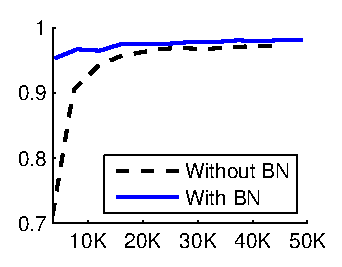
\includegraphics[width=0.28\columnwidth]{mnist.eps}
&
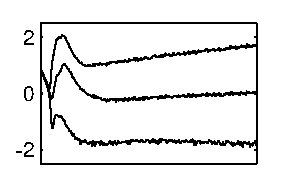
\includegraphics[width=0.35\columnwidth]{evo.eps}&
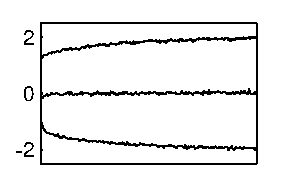
\includegraphics[width=0.35\columnwidth]{evo-bn.eps}\\
(a)&(b) Without BN&(c) With BN
\end{tabular} 
\caption{\em {\em(a)} The test accuracy of the MNIST network trained with and without Batch Normalization, vs. the number of training steps. Batch Normalization helps the network train faster and achieve higher accuracy. {\em(b, c)}   The evolution of input distributions to a typical sigmoid, over the course of training, shown as $\{15, 50, 85\}$th percentiles. Batch Normalization makes the distribution more stable and reduces the internal covariate shift.}
\label{fig-mnist}
\end{figure}

Figure~\ref{fig-mnist}(a) shows the fraction of correct predictions  by the two networks on
held-out test data, as training progresses. The batch-normalized network enjoys the higher test accuracy. To investigate why, we studied inputs to the sigmoid, in the original network $\norig$ and  batch-normalized network $\ntrain$ (Alg.~\ref{alg-train}) over the course of training. In Fig.~\ref{fig-mnist}(b,c) we show, for one typical activation from the last hidden layer of each network, how its distribution evolves.  The distributions in the original network
change significantly over time, both in their mean and the variance, which complicates the training of the subsequent layers.  In
contrast, the distributions in the batch-normalized network are much more stable
as training progresses, which aids the training.


\subsection{ImageNet classification}
\label{sec-results}

We applied Batch Normalization to a new variant of the Inception network \cite{inception},
trained on the ImageNet classification task \cite{imagenet}. The network has a large
number of convolutional and pooling layers, with a softmax layer to predict the
image class, out of 1000 possibilities. Convolutional layers use ReLU as the
nonlinearity. The main difference to the network described in \cite{inception} is that
the $5\times 5$ convolutional layers are replaced by two consecutive layers of $3\times 3$ convolutions
with up to $128$ filters. The network contains $13.6\mils$ parameters, and, other than the top softmax layer, has no fully-connected layers.  More details are given in the Appendix.  We refer to this model as {\sl Inception} in the rest of the text. The model was trained using a version of Stochastic Gradient Descent with momentum
\cite{momentum}, using the mini-batch size of 32. The training was performed using a large-scale, distributed architecture (similar to \cite{dist-belief}).
All networks are evaluated as training progresses by computing the validation accuracy $@1$, i.e. the
probability of predicting the correct label out of 1000 possibilities, on a held-out set, using a single crop per image.

\begin{figure*}
\centering
\begin{minipage}[b]{\columnwidth}
\begin{tabular}{@{}c@{}}
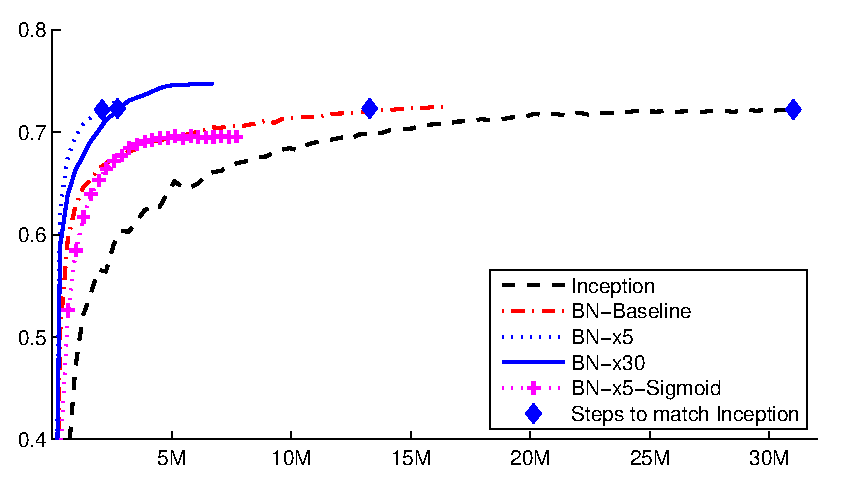
\includegraphics[width=\columnwidth]{inception-compare.eps}
\end{tabular} 
\caption{\em Single crop validation accuracy of Inception and its
  batch-normalized variants, vs. the number of training steps.  }
\label{fig-inception}
\end{minipage}
\qquad
%
\begin{minipage}[b]{0.9\columnwidth}
\begin{tabular}{@{} c | r  r  @{}}
\hline
Model & Steps to  72.2\% & Max accuracy \\ 
\hline
Inception& $31.0\mils$ & 72.2\%  \\
\sl BN-Baseline& $13.3\mils$ & 72.7\%  \\
\sl BN-x5& $2.1\mils$ & 73.0\%  \\
\sl BN-x30& $2.7\mils$ & 74.8\% \\
\sl BN-x5-Sigmoid&  & 69.8\%\\\hline
\end{tabular}
\caption{\em For Inception and the batch-normalized variants, the number of training steps required to reach the maximum accuracy of Inception (72.2\%), and the maximum accuracy achieved by the network.}
\label{fig-stats}
\end{minipage}
\end{figure*}

In our experiments, we evaluated several modifications of Inception with Batch Normalization. In all cases, Batch Normalization was applied to the 
input of each nonlinearity, in a convolutional way, as described in section
\ref{sec-conv}, while keeping the rest of the architecture constant.

\subsubsection{Accelerating BN Networks}
\label{sec-accelerating}
Simply adding Batch Normalization to a network does not take full advantage of our method. To do so, we further changed the network and its training parameters, as follows:

{\em Increase learning rate.} In a batch-normalized model, we have been able to achieve a training speedup from higher learning rates, with no ill side effects (Sec.~\ref{sec-lr}).

 {\em Remove Dropout.} As described in Sec.~\ref{sec-regularizer}, Batch Normalization fulfills some of the same goals as Dropout. Removing Dropout from Modified BN-Inception speeds up training, without increasing overfitting. 
 
{\em Reduce the $L_2$ weight regularization.} While in Inception an $L_2$ loss on the model parameters controls overfitting, in Modified BN-Inception the weight of this loss is reduced by a factor of 5. We find that this improves the accuracy on the held-out validation data.

{\em Accelerate the learning rate decay.} In training Inception, learning rate was decayed exponentially. Because our network trains faster than Inception, we lower the learning rate  6 times faster.

{\em Remove Local Response Normalization}   While Inception and other networks \cite{dropout} benefit from it, we found that with Batch Normalization  it is not necessary.

{\em Shuffle training examples more thoroughly.} We enabled within-shard shuffling of the training data, which prevents the same examples from always appearing in a mini-batch together. This  led to about 1\% improvements in the validation accuracy, which is consistent with the view of Batch Normalization as a regularizer (Sec.~\ref{sec-regularizer}): the randomization inherent in our method should be most beneficial when it  affects an example differently each time it is seen.

{\em Reduce the photometric distortions.} Because batch-normalized networks train faster and observe each training example fewer times, we let the trainer focus on more ``real'' images by distorting them less.

\subsubsection{Single-Network Classification}

We evaluated the following networks, all trained on the LSVRC2012 training data, and tested on the validation data:


\netw{Inception}: the network described at the beginning of Section \ref{sec-results}, trained with the initial learning rate of 0.0015.

\netw{BN-Baseline}: Same as Inception with Batch Normalization before each nonlinearity.

\netw{BN-x5}: Inception with Batch Normalization and the modifications  in Sec.~\ref{sec-accelerating}. The initial learning rate was increased by a factor of 5, to 0.0075. The same learning rate increase with original Inception caused the model parameters to reach machine infinity.

\netw{BN-x30}: Like \netw{BN-x5}, but with the initial learning rate  0.045 (30 times that of Inception).

\netw{BN-x5-Sigmoid}: Like \netw{BN-x5}, but with sigmoid nonlinearity $g(t)=\frac{1}{1+\exp(-x)}$ instead of ReLU.
We also attempted to train the original Inception with sigmoid, but the model remained at the  accuracy equivalent to chance.

In Figure~\ref{fig-inception}, we show the validation accuracy of the
networks, as a function of the number of training steps.  Inception
reached the accuracy of 72.2\% after $31\mils$ training steps. The
Figure~\ref{fig-stats} shows, for each network, the number of training
steps required to reach the same 72.2\% accuracy, as well as the
maximum validation accuracy reached by the network and the number of steps
to reach it.
 
By only using Batch Normalization (\netw{BN-Baseline}), we match the accuracy of Inception in less than half the number of training steps. By applying the modifications in Sec.~\ref{sec-accelerating}, we significantly increase the training speed of the network. \netw{BN-x5} needs 14 times fewer steps than Inception to reach the 72.2\% accuracy.
Interestingly, increasing the learning rate further (\netw{BN-x30})  causes the model to train somewhat {\em slower} initially, but allows it to reach a higher final accuracy. It  reaches  74.8\% after $6\mils$ steps, i.e. 5 times fewer steps than required by Inception to reach 72.2\%.

We also verified that the  reduction in internal covariate shift allows deep networks with Batch Normalization to be trained when sigmoid is used as the nonlinearity, despite the well-known difficulty of training such networks. Indeed, \netw{BN-x5-Sigmoid} achieves the accuracy of  69.8\%. Without Batch Normalization, Inception with sigmoid never achieves better than $1/1000$ accuracy.

\subsubsection{Ensemble Classification}

\begin{figure*}[t!]
\centering
\begin{tabular}{c | r  r  r  r  r }
\hline
Model & Resolution & Crops & Models & Top-1 error & Top-5 error \\ 
\hline
{GoogLeNet ensemble} & 224 & 144 & 7 & - & 6.67\% \\
{Deep Image low-res} & 256 & - & 1 & - & 7.96\% \\
{Deep Image high-res} & 512 & - & 1 & 24.88 & 7.42\% \\
{Deep Image ensemble} & variable & - & - & - & 5.98\% \\
{BN-Inception single crop} & 224 & 1 & 1 & 25.2\% & 7.82\% \\
{BN-Inception multicrop} & 224 & 144 & 1 & 21.99\% & 5.82\% \\
{BN-Inception ensemble} & 224 & 144 & 6 & 20.1\% & {\bf 4.9\%}* \\
\hline
\end{tabular}
\caption{\em Batch-Normalized Inception comparison with previous state of the art on the provided validation set comprising 50000 images.
  *BN-Inception ensemble has reached 4.82\% top-5 error on the 100000 images of the test set of the ImageNet as reported by the test server. }
\label{fig-classification-comparison}
\end{figure*}

The current reported best results on the ImageNet Large Scale Visual Recognition
Competition are reached by the Deep Image ensemble of traditional models
\cite{deepimage} and the ensemble model of \cite{msr}. The latter reports the
top-5 error of 4.94\%, as evaluated by the ILSVRC server. Here we report a top-5
validation error of 4.9\%, and test error of 4.82\% (according to the ILSVRC
server). This improves upon the previous best result,
% despite using 15X fewer parameters than Deep Image and lower resolution receptive field. Our system
and
exceeds the estimated accuracy of human raters according to \cite{imagenet}.

%% jan16.pyplan/train_nbl0_lrmult6_wmp1
%% jan16.pyplan/train_lrmult6_wmp0_drop10
%% jan16.pyplan/train_lrmult6_wmp2_drop5
%% jan17.pyplan/train_nbl1_lrmult6_wmp1
%% jan17.pyplan/train_nbl1_lrmult6_wmp2
%% jan17.pyplan/train_nbl2_lrmult6_wmp1

For our ensemble, we used 6 networks. Each was based on {\sl BN-x30},
modified via some of the following: increased initial weights in the
convolutional layers; using Dropout (with the Dropout probability of
5\% or 10\%, vs. 40\% for the original Inception); and using
non-convolutional, per-activation Batch Normalization with last hidden
layers of the model. Each network achieved its maximum accuracy after
about $6\mils$ training steps.  The ensemble prediction was based on
the arithmetic average of class probabilities predicted by the
constituent networks. The details of ensemble and multicrop inference
are similar to \cite{inception}.

We demonstrate in Fig.~\ref{fig-classification-comparison} that batch
normalization allows us to set new state-of-the-art by a healthy
margin on the ImageNet classification challenge benchmarks.

\section{Conclusion}

We have presented a novel mechanism for dramatically accelerating the
training of deep networks. It is based on the premise that covariate
shift, which is known to complicate the training of machine learning
systems, also applies to sub-networks and layers, and removing it from
internal activations of the network may aid in training. Our proposed
method draws its power from normalizing activations, and from
incorporating this normalization in the network architecture
itself. This ensures that the normalization is appropriately handled
by any optimization method that is being used to train the network. To
enable stochastic optimization methods commonly used in deep network
training, we perform the normalization for each mini-batch, and
backpropagate the gradients through the normalization
parameters. Batch Normalization adds only two extra parameters per
activation, and in doing so preserves the representation ability of
the network. We presented an algorithm for constructing, training, and
performing inference with batch-normalized networks. The resulting
networks can be trained with saturating nonlinearities, are more
tolerant to increased training rates, and often do not require Dropout
for regularization.

Merely adding Batch Normalization to a state-of-the-art image
classification model yields a substantial speedup in training. By
further increasing the learning rates, removing Dropout, and applying
other modifications afforded by Batch Normalization, we reach the
previous state of the art with only a small fraction of training steps
-- and then beat the state of the art in single-network image
classification. Furthermore, by combining multiple models trained with
Batch Normalization, we perform better than the best known system on
ImageNet, by a significant margin.


Interestingly, our method bears similarity to the standardization layer of
\cite{gulcehre}, though the two methods stem from very different goals, and
perform different tasks. The goal of Batch Normalization is to achieve a stable
distribution of activation values throughout training, and in our experiments we
apply it before the nonlinearity since that is where matching the first and
second moments is more likely to result in a stable distribution. On the
contrary, \cite{gulcehre} apply the standardization layer to the {\em output} of
the nonlinearity, which results in sparser activations. In our large-scale image
classification experiments, we have not observed the nonlinearity {\em inputs}
to be sparse, neither with nor without Batch Normalization. Other notable
differentiating characteristics of Batch Normalization include the learned scale
and shift that allow the BN transform to represent identity (the standardization
layer did not require this since it was followed by the learned linear transform
that, conceptually, absorbs the necessary scale and shift), handling of
convolutional layers, deterministic inference that does not depend on the
mini-batch, and batch-normalizing each convolutional layer in the network.


In this work, we have not explored the full range of possibilities
that Batch Normalization potentially enables. Our future work includes
applications of our method to Recurrent Neural Networks
\cite{pascanu-rnn}, where the internal covariate shift and the
vanishing or exploding gradients may be especially severe, and which
would allow us to more thoroughly test the hypothesis that
normalization improves gradient propagation (Sec.~\ref{sec-lr}). We
plan to investigate whether Batch Normalization can help with domain
adaptation, in its traditional sense -- i.e. whether the normalization
performed by the network would allow it to more easily generalize to
new data distributions, perhaps with just a recomputation of the
population means and variances (Alg.~\ref{alg-train}). Finally, we
believe that further theoretical analysis of the algorithm would allow
still more improvements and applications.


\bibliography{bnicml}
\bibliographystyle{icml2015}


\section*{Appendix}
\subsection*{Variant of the Inception Model Used}
\begin{figure*}[b]
{\small
\begin{center}
  \begin{tabular}[H]{@{}|l|c|c|c|c|c|c|c|c|c|}
\hline
{\bf type} & {\bf \stackanchor{patch size/}{stride}} & {\bf \stackanchor{output}{size}} &
{\bf depth} & {\bf $\#1{\times}1$} & {\bf \stackanchor{$\#3{\times}3$}{reduce}} & $\#3{\times}3$ &
{\bf \stackanchor{double $\#3{\times}3$}{reduce}} & {\bf \stackanchor{double}{ $\#3{\times}3$}} & {\bf Pool +proj} \\
\hline\hline
convolution* & $7{\times}7/2$ & $112{\times}112{\times}64$ & 1 & & & & & & \\
\hline
max pool & $3{\times}3/2$ & $56{\times}56{\times}64$ & 0 & & & & & & \\
\hline
convolution & $3{\times}3/1$ & $56{\times}56{\times}192$ & 1 & & 64 & 192 & & &  \\
\hline
max pool & $3{\times}3/2$ & $28{\times}28{\times}192$ & 0 & & & & & & \\
\hline
inception (3a) & & $28{\times}28{\times}256$ & 3 & 64 & 64 & 64 & 64 & 96 & avg + 32  \\
\hline
inception (3b) & & $28{\times}28{\times}320$ & 3 & 64 & 64 & 96 & 64 & 96 & avg + 64 \\
\hline
inception (3c) & stride 2 & $28{\times}28{\times}576$ & 3 & 0 & 128 & 160 & 64 & 96 & max + pass through \\
\hline
inception (4a) & & $14{\times}14{\times}576$ & 3 & 224 & 64 & 96 & 96 & 128 & avg + 128 \\
\hline
inception (4b) & & $14{\times}14{\times}576$ & 3 & 192 & 96 & 128 & 96 & 128 & avg + 128 \\
\hline
inception (4c) & & $14{\times}14{\times}576$ & 3 & 160 & 128 & 160 & 128 & 160 & avg + 128 \\
\hline
inception (4d) & & $14{\times}14{\times}576$ & 3 & 96 & 128 & 192 & 160 & 192 & avg + 128 \\
\hline
inception (4e) & stride 2 & $14{\times}14{\times}1024$ & 3 & 0 & 128 & 192 & 192 & 256 & max + pass through \\
\hline
inception (5a) & & $7{\times}7{\times}1024$ & 3 & 352 & 192 & 320 & 160 & 224 & avg + 128 \\
\hline
inception (5b) & & $7{\times}7{\times}1024$ & 3 & 352 & 192 & 320 & 192 & 224 & max + 128 \\
\hline
avg pool & $7{\times}7/1$ & $1{\times}1{\times}1024$ & 0 & & & & & & \\
\hline
  \end{tabular}
\end{center}
}
\caption{Inception architecture}
\label{fig-arch}
\end{figure*}

Figure~\ref{fig-arch} documents the changes that were performed compared to the architecture with respect to the GoogleNet archictecture. For the interpretation of this table, please consult \cite{inception}. The notable architecture changes compared to the GoogLeNet model include:
\begin{itemize}
\item The 5${\times}$5 convolutional layers are replaced by two consecutive 3${\times}$3 convolutional layers. This increases the maximum depth of the network by 9 weight layers. Also it increases the number of parameters by 25\% and the computational cost is increased by about 30\%.
\item The number 28${\times}$28 inception modules is increased from 2 to 3.
\item Inside the modules, sometimes average, sometimes maximum-pooling is employed. This is indicated in the entries corresponding to the pooling layers of the table.
\item There are no across the board pooling layers between any two Inception modules, but stride-2 convolution/pooling layers are employed before the filter concatenation in the modules 3c, 4e.
\end{itemize}
Our model employed separable convolution with depth multiplier $8$ on the first convolutional layer. This reduces the computational cost while increasing the memory consumption at training time.


\end{document}
